\documentclass[cyan]{elegantnote}
\author{Yuyang Songsheng}
\email{songshengyuyang@gmail.com}
\zhtitle{物理}
\entitle{Physics}
\version{1.00}
\myquote{Summary is the best way to say "Good Bye"}
\logo{logo.jpg}
\cover{cover.pdf}
%green color
   \definecolor{main1}{RGB}{210,168,75}
   \definecolor{seco1}{RGB}{9,80,3}
   \definecolor{thid1}{RGB}{0,175,152}
%cyan color
   \definecolor{main2}{RGB}{239,126,30}
   \definecolor{seco2}{RGB}{0,175,152}
   \definecolor{thid2}{RGB}{236,74,53}
%cyan color
   \definecolor{main3}{RGB}{127,191,51}
   \definecolor{seco3}{RGB}{0,145,215}
   \definecolor{thid3}{RGB}{180,27,131}

\usepackage{mhchem}
\usepackage{makecell}
\usepackage{lipsum}
\usepackage{amssymb}
\usepackage{float}
\usepackage{wrapfig}
\usepackage{latexsym}
\usepackage{hyperref}
\usepackage{feynmf}
\usepackage{exscale}
\usepackage{relsize}
\usepackage{slashed}
\usepackage{bm}%bold math, for vector


\begin{document}
\maketitle
\tableofcontents

\chapter{Systems with Interaction and Quantum Field Theory}
\section{Superfluidity}
\subsection{Experimental facts of Helium at low temperatures}
Helium is the only element which remains a liquid at zero temperature and atmospheric pressure.
Experimentally the phase diagram of \ce{^{4}He} is shown in Figure below.
\begin{figure}[!h]
\centering
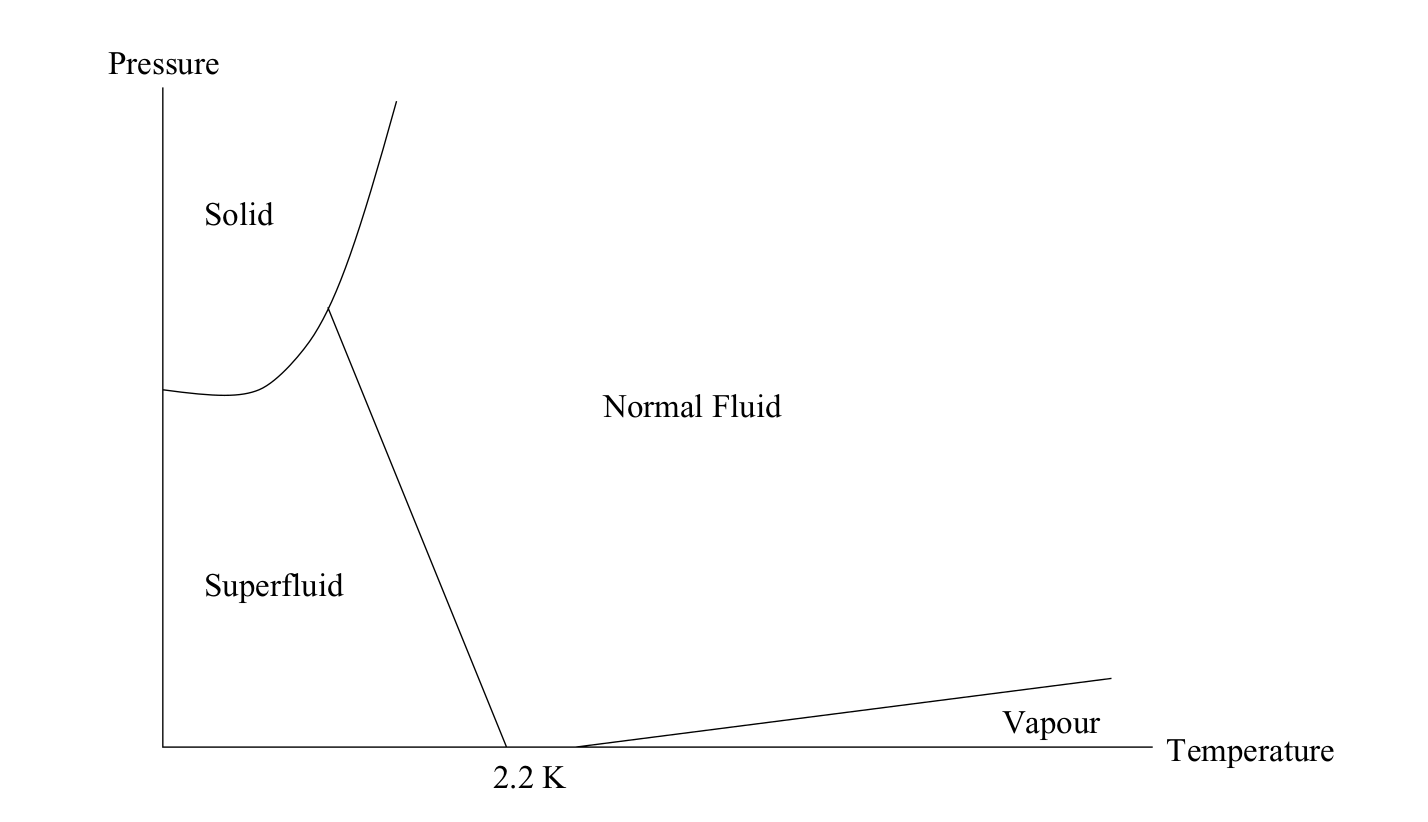
\includegraphics[scale=0.15]{SM/He1.png}
\caption{The phase structure of \ce{^{4}He} at low temperature}
\end{figure}
Helium I is a normal fluid and has a normal gas-liquid critical point. Helium II is a mixture of a normal fluid and a superfluid. 
The superfluid is characterized by the vanishing of its viscosity. Helium I and helium II are separated by a line known as the $\lambda$-transition line.  At $T_{\lambda} = 2.18\mathrm{K}$, $P_{\lambda} = 2.29\mathrm{Pa}$, helium I, helium II, and helium gas coexist. 
The specific heat of liquid helium along the vapour transition line forms a logarithmic discontinuity. The form of this diagram resembles the Greek letter $\lambda$ and is the reason for calling the transition a $\lambda$ transition.
\begin{figure}[!h]
\centering
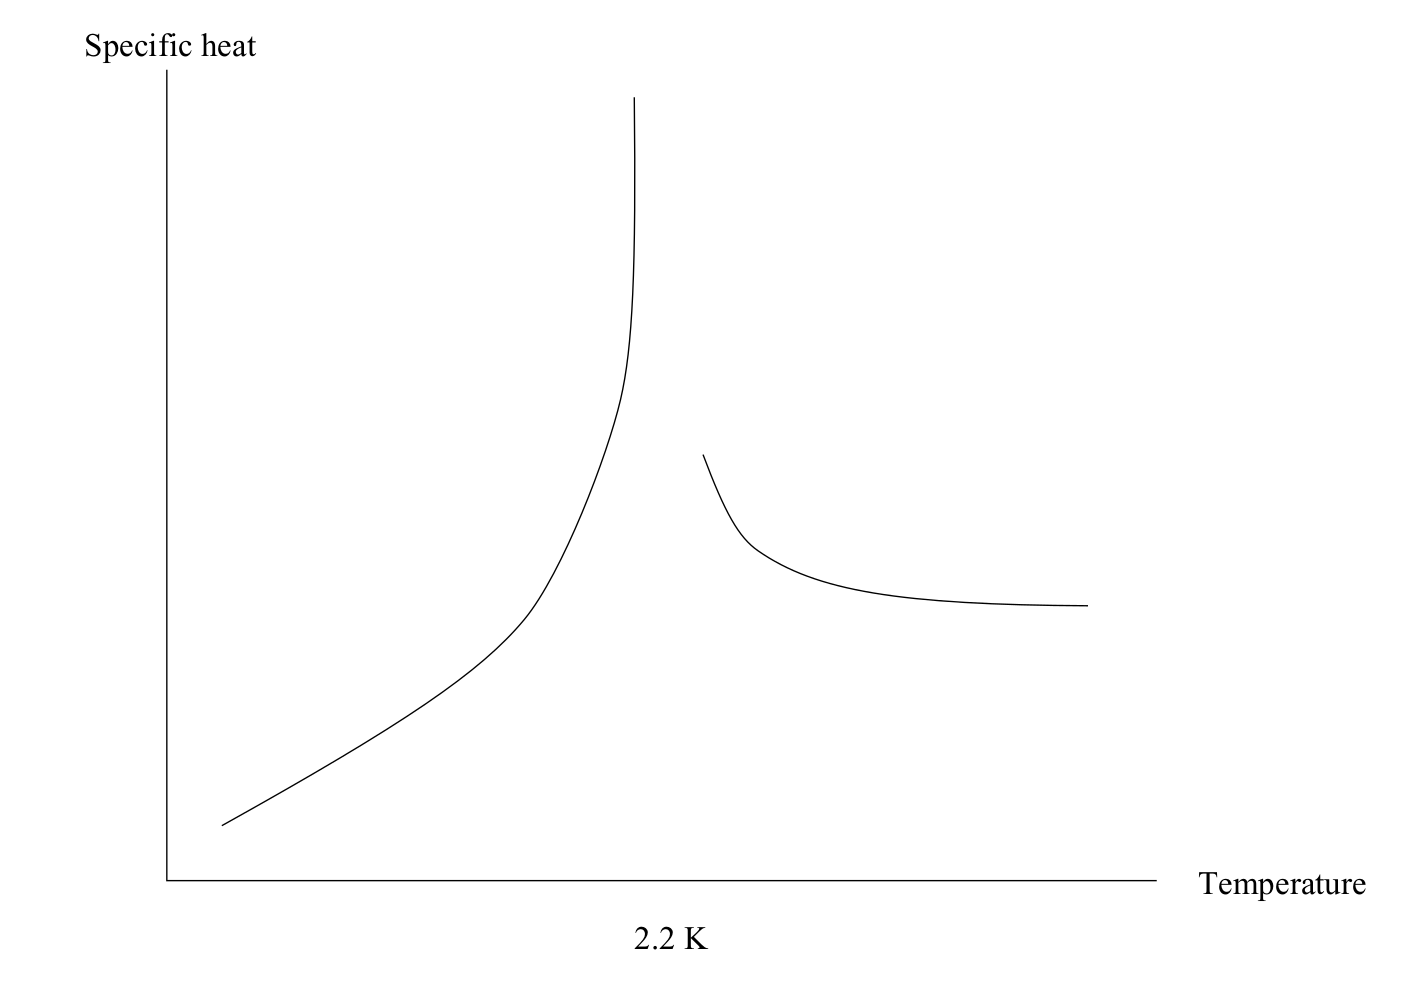
\includegraphics[scale=0.12]{SM/He2.png}
\caption{The specific heat of helium as a function of temperature}
\end{figure}
\\
The excitation spectrum of helium II can be measured experimentally through elastic neutron scattering. It is found to consist of two parts, the phonon region
\[E(\bm{p}) = c|\bm{p}| \quad \mbox{ when } |\bm{p}| \ll |\bm{p}_0|\]
and the roton region
\[E(\bm{p}) = \Delta + \frac{1}{2\mu} |\bm{p} - \bm{p}_0|^2 \quad \mbox{ when } |\bm{p}| \sim |\bm{p}_0|\]
where $c = 226 \mathrm{m/s}$ is the velocity of sound, $\Delta/k_B = 9\mathrm{K}$ are the roton parameters, and $\mu = 0.25m_{He}$. 
There is another velocity parameter known as the critical velocity $v_0$. It is only when helium II moves with velocity greater than $v_0$ that viscous effects arise. At low temperature the roton excitations are damped by the Boltzmann factor $\exp(-\beta \Delta)$.

\subsection{Quantum field theory formulation}
Recall the non-relativistic quantum field theory we develop in quantum mechanics.
The Hamiltonian of a system of \ce{^{4}He} in momentum space is
\[H = \sum_{\bm{k}} \frac{|\bm{k}|^2}{2m} a_{\bm{k}}^{\dagger} a_{\bm{k}} + \frac{1}{2V} \sum_{\bm{k}_1,\bm{k}_2,\bm{q}} \tilde{V}(\bm{q}) a^{\dagger}_{\bm{k}_1 + \bm{q}} a^{\dagger}_{\bm{k}_2-\bm{q}} a_{\bm{k}_1} a_{\bm{k}_2}\]
where
\[a_{\bm{k}} = \frac{1}{\sqrt{V}} \int d\bm{x}\psi(\bm{x}) e^{-i\bm{p}\cdot\bm{x}}\]
and
\[\tilde{V}(\bm{q}) = \int d\bm{x} V(\bm{x}) e^{-i\bm{q}\cdot\bm{x}}\]
Here we adopt box normalization to make momentum of the particle discrete. It is easy to verify that
\[[a_{\bm{p}},a_{\bm{q}}^{\dagger}] = \delta_{\bm{p},\bm{q}} \quad [a_{\bm{p}},a_{\bm{q}}] = 0 \quad [a^{\dagger}_{\bm{p}},a^{\dagger}_{\bm{q}}] = 0\]
The partition canonical partition function is
\[Z = \mathrm{Tr}[e^{-\beta H}]\]
At low temperature, states with low energy value become dominant. These are expected to be states with low values of momentum. 
Let us consider the system close to $T \approx 0$. 
We can then assume that the state of lowest energy corresponds to atoms of low momentum with a sizable fraction of molecules in the zero momenta state, leading to Bose-Einstein condensation. 
Thus if the system has on average $N$ atoms then a significant number $N_0$ of the atoms are in the lowest energy state. More precisely we suppose that the ratio $N_0 / N$ converges to a constant in the limit $N \to \infty$. 
Let us suppose that $|C;N,N_0\rangle$ is a superfluid state with a total of $N$ helium atoms, $N_0$ of which are in the zero momentum plane wave state. 
If $a_0^{\dagger}$ and $a_0$ are creation and destruction operators for a state of zero momentum, we have
\[a_0^{\dagger}a_0 |C;N,N_0\rangle = N_0 |C;N,N_0\rangle\]
and
\[a_0a_0^{\dagger} |C;N,N_0\rangle = (N_0+1) |C;N,N_0\rangle\]
For large $N_0$ we can approximate $N_0 + 1$ by $N_0$ so that on the state $|C;N,N_0\rangle$ we can replace both the operators $a_0^{\dagger}a_0$ and $a_0^{\dagger}a_0$ by a single c-number, $N_0$.

\subsection{The quasi-particle approach}
For $|C;N,N_0\rangle$, the particle number operator $\hat{N}$ can be written as
\[\hat{N} = N_0 + \sum_{\bm{k}\neq 0}a_{\bm{k}}^{\dagger} a_{\bm{k}} \]
Neglecting terms of order $O(N_0^0)$, we have
\[N^2 \approx N_0^2 + 2N_0\sum_{\bm{k}\neq 0}a_{\bm{k}}^{\dagger} a_{\bm{k}} \]
We next examine the interaction part of $H$ when restricted to $|C\rangle$. When all four operators in H I have zero momentum, we have the term
\[H_I^0 = \frac{1}{2V} \tilde{V}(0) a^{\dagger}_{0} a^{\dagger}_{0} a_{0} a_{0} = \frac{1}{2V}\tilde{V}(0)N_0^2 \approx  \frac{1}{2V}\tilde{V}(0) \left[\hat{N}^2-2N_0\sum_{\bm{k}\neq 0}a_{\bm{k}}^{\dagger} a_{\bm{k}} \right]\]
The next term is of order $N_0$ and is the part of $H_I$ containing two operators (carrying zero momentum). There are six ways in which this can happen. If we make an additional assumption that, for $|\bm{k}|$ small, $\tilde{V}(\bm{k}) = \tilde{V}(0)$. 
Since at low temperature we expect only small momenta excitations to be important we replace $\tilde{V}(\bm{k})$ by $\tilde{V}(0)$ in $H_I$. Therefore, on the state , the interacting Hamiltonian, keeping terms of $O(N_0)$ is given by
\[H_I \approx \tilde{V}(0) \left\{ \frac{1}{2V}\left[N^2-2N_0\sum_{\bm{k}\neq 0}a_{\bm{k}}^{\dagger} a_{\bm{k}} \right]  +\frac{N_0}{2V}\sum_{\bm{k}\neq 0} [a^{\dagger}_{\bm{k}} a^{\dagger}_{-\bm{k}} + a_{\bm{k}} a_{-\bm{k}}] +\frac{2N_0}{V} \sum_{\bm{k}\neq 0}a_{\bm{k}}^{\dagger} a_{\bm{k}} \right\} \equiv H_I^B \] 
and the total Hamiltonian can be approximated by the Bogoliubov Hamiltonian $H_B$ given by
\[H^B = \sum_{\bm{k}} \frac{|\bm{k}|^2}{2m} a_{\bm{k}}^{\dagger} a_{\bm{k}} + H_I^B = \sum_{\bm{k}\neq 0} \left(\frac{|\bm{k}|^2}{2m} + \frac{\tilde{V(0)}}{V}N_0 \right)a_{\bm{k}}^{\dagger} a_{\bm{k}}  + \frac{\tilde{V}(0)N_0}{2V} \sum_{\bm{k}\neq 0} [a^{\dagger}_{\bm{k}} a^{\dagger}_{-\bm{k}} + a_{\bm{k}} a_{-\bm{k}}]\]
\\
We turn next to the problem of determining the energy eigenvalues of this Hamiltonian. This we do by using the method of the Bogoliubov–Valatin transform. 
The idea is this: $H_B$ is a quadratic function of the operators $a_{\bm{k}}$ and $a^{\dagger}_{\bm{k}}$. 
By taking appropriate linear combinations of these operators we can form new operators $b_{\bm{k}}$ and $b^{\dagger}_{\bm{k}}$ which "diagonalize" $H^B$, i.e. which lead to
\[H^B = \sum_{\bm{q} \neq 0} \mathcal{E}(\bm{k})b^{\dagger}_{\bm{k}} b_{\bm{k}} \]
The function $\mathcal{E}(\bm{k})$  will then determine the different excitations of the system while $b_{\bm{k}}$ and $b^{\dagger}_{\bm{k}}$ will be destruction and creation operators for these excitations or "quasi-particles", provided they satisfy the commutation rules
\[[b_{\bm{p}},b_{\bm{q}}^{\dagger}] = \delta_{\bm{p},\bm{q}}\]
We write
\[b_{\bm{k}} = \alpha(\bm{k})a_{\bm{k}} - \beta(\bm{k})a^{\dagger}_{-\bm{k}} \quad b^{\dagger}_{\bm{k}} = \alpha(\bm{k})a^{\dagger}_{\bm{k}} - \beta(\bm{k})a_{-\bm{k}} \]
And we have the constraint
\[\alpha(\bm{k})^2 - \beta(\bm{k})^2 = 1\]
Substituting $a$ and $a^{\dagger}$ with $b$ and $b^{\dagger}$ in $H^B$ and comparing it with the $\sum_{\bm{q} \neq 0} \mathcal{E}(\bm{k})b^{\dagger}_{\bm{k}} b_{\bm{k}}$, we can can a set of equations of $\alpha(\bm{k})$ and $\beta(\bm{k})$. Finally, we have
\[\mathcal{E}(\bm{k}) = \sqrt{\frac{\bm{k}^2}{2m} \left(\frac{\bm{k}^2}{2m} + \frac{2N_0\tilde{V}(0)}{V} \right) }\]
The energy $\mathcal{E}(\bm{k})$ is called the quasi-particle energy and the operators $b_{\bm{k}}$ and $b^{\dagger}_{\bm{k}}$ are quasi-particle destruction and creation operators. 
For small values of $\bm{k}$ we have
\[\mathcal{E}(\bm{k}) = \frac{|\bm{p}|}{m} \sqrt{\frac{N_0}{V}\tilde{V}(0)m}\]
Observe that for $\mathcal{E}(\bm{k})$ to be real we must have $\tilde{V}(0) > 0$. This implies there is a repulsive region for $V(x)$ which must dominate the integral $\int dx V(x)$. Observe also that $|\bm{k}|/m = \bm{v}$ is a velocity, and $N_0m/V = \rho$, is the density of the superfluid helium so that the quasi-particle energy can be written as 
\[\mathcal{E}(\bm{p} = m\bm{v}) \approx |\bm{v}|\sqrt{\rho\tilde{V}(0)}\]
\\
We now show that a system with such an energy spectrum represents a superfluid, i.e. a system with no friction.
Friction in a system represents dissipation of energy.
Consider a molecule of mass $M_A$ moving in a medium. If this molecule can change its energy through collisions with the excitations of the medium, then the system has friction. 
We will find that a molecule of mass $M_A$ and velocity $\bm{V}_A$ moving through a system consisting of quasi-particles of energy $\mathcal{E}(\bm{k})$ cannot change its energy by scattering off quasi-particles if $|\bm{V}_A| < |\bm{v}_0|$ where $|\bm{v}_0|$ is a critical velocity determined by $\tilde{V}(0)$ and $\rho$. 
Thus for $|\bm{V}_A| < |\bm{v}_0|$ the system of quasi-particles behaves as a frictionless superfluid.
\\
To see this, let us consider the collision of a molecule of mass $M_A$ and velocity $\bm{V}_A$ with a quasi-particle at rest. If the final momentum of the molecule is $\bm{Q}_A$ and that of the quasi-particle is $\bm{k}$, we have, from momentum conservation,
\[|\bm{Q}_A|^2 = |\bm{P}_A|^2 + |\bm{k}|^2 - 2|\bm{P}_A||\bm{k}|\cos\theta\]
We then have
\[\frac{|\bm{P}_A|^2-|\bm{Q}_A|^2}{2|\bm{P}_A| |\bm{k}|} \leq \frac{|\bm{P}_A|^2-|\bm{Q}_A|^2 + |\bm{k}|^2}{2|\bm{P}_A| |\bm{k}|} = \cos\theta \leq 1\]
Combining this with the energy conservation condition
\[\frac{|\bm{Q}_A|^2}{2M_A} = \frac{|\bm{P}_A|^2}{2M_A} + \mathcal{E}(\bm{p})\]
we end up with
\[\frac{M_A\mathcal{E}(\bm{k})}{|\bm{P}_A| |\bm{k}|} = \frac{1}{m}\sqrt{\frac{\tilde{V}(0)N_0m}{V}} \frac{1}{V_A} \leq 1\]
Thus the process of changing energy for the molecule is not allowed if $V_A \leq v_0 = \frac{1}{m}\sqrt{\frac{\tilde{V}(0)N_0m}{V}} $ and the system of quasi-particles behaves like a superfluid.

\section{Finite temperature perturbation theory}
In this section we develop a perturbative formalism for the computation of the grand canonical partition function. This proceeds in close analogy with the perturbative evaluation of the evolution operator. The grand canonical partition sum 
\[Z_{\Omega} = \mathrm{Tr}e^{-\beta K}\]
where
\[K \equiv K_0 + H_{\mathrm{int}} \equiv H_0 + H_{\mathrm{int}} -\mu N\]
Define
\[U(\beta) \equiv \exp(-\beta K) \quad U_0(\beta) \equiv \exp(-\beta K_0) \quad W(\beta) = U_0^{\dagger}(\beta)U(\beta)\]
Similar to the time-dependent perturbation theory in quantum mechanics, we can get
\[\frac{\partial W}{\partial \beta} = -H_I(\beta)W(\beta)\]
where
\[H_I(\beta) = U_0^{\dagger}(\beta)H_{\mathrm{int}}U_0(\beta)\]
The solution of the equation above can be represented by Dyson series
\[W(\beta) = \sum_{n \geq 0} \frac{(-1)^n}{n!} \int_0^{\beta}d\tau_1 \cdots \int_0^{\beta} d\tau_n T[H_I(\tau_1)\cdots H_I(\tau_n)]\]
Note that $T$ is now the ordering with respect to $\tau$ (or imaginary time). Finally, upon substitution of this last expression into the grand canonical partition sum
\[Z_{\Omega} = \mathrm{Tr} e^{-\beta K_0}W(\beta)\]
we obtain a perturbative expansion of the partition sum in analogy with that of the evolution operator. Before we can apply this formalism to the computation of $Z_{\Omega}$ we need to analyze the finite temperature versions of the time-ordered Green functions and Wick's theorem. The detailed discussion can be found in section 9.8 from \emph{Elements Of Statistical Mechanics (ivo Sachs, Siddhartha Sen, James Sexton)}.

\section{Path integrals}
Similar to the time evolution operator in quantum mechanics, the partition function can be calculated through path integral. We firstly note that
\[e^{-\epsilon(T+V)} = e^{-\frac{\epsilon}{2} V}e^{-\epsilon T} e^{-\frac{\epsilon}{2} V} + O(\epsilon^3)\]
So if we define
\[\epsilon \equiv \frac{\beta}{n}\]
we have
\[\mathrm{Tr}e^{-\beta H} = \mathrm{Tr} \left( e^{-\epsilon H} \right)^n = \mathrm{Tr} \left(e^{-\frac{\epsilon}{2} V}e^{-\epsilon T} e^{-\frac{\epsilon}{2} V}\right)^n + nO(\epsilon^3) = \mathrm{Tr} \left(e^{-\epsilon V}e^{-\epsilon T} \right)^n + O(\epsilon^2)\]
In the limit $n \to \infty$ the error term will go to zero, and we have achieved a splitting of the original exponential operator
\[\mathrm{Tr}e^{-\beta H} = \lim_{n \to \infty} \mathrm{Tr} \left(e^{-\epsilon V}e^{-\epsilon T} \right)^n\]
At this point we are still working with operators, but we can now insert a complete set of states between each term in the product, and convert the problem to one with just commuting numbers. For simplicity, we assume the system has only one pair of canonical variables.
\begin{eqnarray}
&\phantom{=}& \mathrm{Tr}e^{-\beta H} \nonumber \\
&=& \lim_{n \to \infty} \int [dpdq]^n  \mathrm{Tr} [ e^{-\epsilon V}|q_0\rangle \langle q_0 | e^{-\epsilon T} |p_0 \rangle\langle p_0| e^{-\epsilon V} \cdots e^{-\epsilon V} |q_{n-1}\rangle\langle q_{n-1}| e^{-\epsilon T} |p_{n-1}\rangle\langle p_{n-1} | ] \nonumber \\
&=& \lim_{n \to \infty} \int [\frac{dpdq}{2\pi}]^n e^{\sum_{i=0}^{n-1}ip_i(x_{i+1}-x_i) - \epsilon H(q_i,p_i)} \nonumber
\end{eqnarray}
where $q_{n} = q_0$. 
Generally, we have $T(p) = \frac{p^2}{2m}$. The $p_k$ integral is just a Gaussian integral. The path integral can then be simplified to
\[\mathrm{Tr}e^{-\beta H} = \lim_{n \to \infty} \left( \frac{m}{2\pi \epsilon} \right)^{\frac{n}{2}} \int [dq]^n e^{\epsilon \sum_{i=0}^{n-1}  -\frac{m}{2\epsilon^2}(q_{i+1}-q_i)^2 -  V(q_i)} \]
Similar to path integral formulation in quantum mechanics, the equation above can be written formally as
\[\mathrm{Tr}e^{-\beta H} = \int \mathcal{D}q(\tau) e^{S_E(q(\tau))}\]
with constraint $q(0) = q(\tau)$
where
\[S_E[q(\tau)] = \int_0^{\beta} -\frac{m}{2}\dot{q}^2 - V(q)\]
In quantum mechanics, we have
\[\langle b | e^{-iHT} | a \rangle = \int \mathcal{D}q(t) e^{iS(q(t))}\]
with constraint $q(0) = a$ ans $q(\tau) = b$
where
\[S[q(t)] = \int_0^{T} \frac{m}{2}\dot{q}^2 - V(q)\]
Actually, path integral of quantum mechanics can be obtained directly if we replace $\beta$ with $iT$ and change the integral variable from $\tau$ to $t$ by $\tau = it$ in the path integral  of statistical mechanics.
\\ \\
The path integral formulation can be generalize to the case of quantum field directly. For the system of bosons, we have
\[\mathrm{Tr}e^{-\beta H} = \int \mathcal{D}\psi \mathcal{D}\psi^{\dagger} e^{S_E}\]
with constraint $\psi(\bm{x},0) = \psi(\bm{x},\beta)$
where
\begin{eqnarray}
S_E &=& \int_0^{\beta}d\tau \left[ \int d^3x \psi^{\dagger}(\bm{x},\tau) \left( -\frac{\partial}{\partial \tau} + \frac{\nabla^2}{2m} \right) \psi(\bm{x},\tau) \right. \nonumber \\
&-& \left. \frac{1}{2}\int d^3x d^3y\psi^{\dagger}(\bm{x},\tau)\psi^{\dagger}(\bm{y},\tau)V(\bm{x}-\bm{y})\psi(\bm{x},\tau)\psi(\bm{y},\tau) \right] \nonumber
\end{eqnarray}
As for Fermions, we have
\[\mathrm{Tr}e^{-\beta H} = \int \mathcal{D}\psi \mathcal{D}\psi^{\dagger} e^{S_E}\]
with constraint $\psi(\bm{x},0) = -\psi(\bm{x},\beta)$. 
And the value of $\psi(\bm{x},t)$ is Grassman number rather than $c$ number, which has been discussed in the path integral formulation of Dirac field.

\chapter{Phase Transitions and the Renormalization Group}
\section{Basic problem}
A given equilibrium state of a macroscopic system can be described by an order parameter field. For a ferromagnet the order parameter field is the magnetization density. 
The order parameter field can be regarded as a mapping from the system (with coordinate $\bm{x}$) to an order parameter space. In a model where the magnetization density is given by a scalar function $M_z(\bm{x})$ this is the space of real numbers. In general the order parameter space can be more complicated and the order parameter field need not be a scalar function.
A phase transition corresponds to the order parameter field
changing qualitatively together with the emergence of singular behaviour in the system.
\\ \\
For instance the order parameter field in the case of a ferromagnet is non-zero in the ferromagnetic phase, is zero in the paramagnetic phase, and the susceptibility of the system diverges at the phase transition temperature. 
Determining a suitable order parameter field to characterize a phase is part of the task of a theory of phase transitions. If the order parameter field changes continuously from one phase to another, as in the case of a ferromagnet, the transition is said to be a continuous or second-order phase transition. If it is discontinuous the transition is said to be first order. 
An example of a first order transition is when a solid melts
to a liquid. The density of the system, which can be taken as the order parameter, changes discontinuously. A phase transition is a striking example of an emergent phenomenon. Starting off with only short-range interactions between its microscopic magnetic moments, the system realizes long-range correlations below $T_c$.
\\ \\
We start with a model for a ferromagnet. We regard a ferromagnetic solid as being made out of a finite number of elementary magnets placed at locations throughout the solid.
We simplify our model by assuming that each of these elementary magnets m can either point up $m = 1$ or down $m = -1$. Finally each elementary magnet interacts only with its nearest neighbour. A Hamiltonian for this model could be
\[H = -g\sum_{n,i}m_im_{i+n} - B\sum_i m_i\]
where the first sum is over $i$ as well as the nearest neighbours of $i$. Note $H$ decreases if $m_i$, $m_{i+n}$ have the same sign for $g > 0$. There are altogether a large but finite number of magnets in a ferromagnet. Then we can prove that in the model of a ferromagnet proposed the susceptibility cannot diverge. 
\\
Whereas, the theorem fails if we allow the number of elementary magnets to tend to infinity. This is because an infinite sum of analytic functions need not be analytic. 
In order to analyze this possibility we will need to consider the statistical mechanics partition function in the limit in which the number of configurations is infinite. It is only in this limit that the phase transitions might be understood from this point of view.
\\ \\
Another approach to the problem is to suppose that the external magnetic field $B$ is changed to $B + \delta B(\bm{x})$, i.e. the change $\delta B$ is position dependent. We expect that a change at $\bm{x}$, $\delta B(\bm{x})$, will produce a change in the magnetization $\delta M$ not just at the point $\bm{x}$ but at other points as well. Indeed we might expect
\[\delta M(\bm{y}) \propto C_T(|\bm{x}-\bm{y}|)\delta B(\bm{x})\]
where $C_T$ is a "correlation function" which determines the effect at $\bm{x}$ on the magnetization due to a change in the external field $\delta B$ at $\bm{x}$. The total change
is then expected to be
\[\delta M(\bm{y}) = \int d^3x C_T(|\bm{x}-\bm{y}|)\delta B(\bm{x})\]
We have assumed that the correlation function depends only on temperature and on the distance between the points $\bm{x}$ and $\bm{y}$.
Let us now suppose that $\delta B$ is independent of $\bm{x}$ and let us set $\bm{y} = 0$. Then we have
\[\chi(0) = \frac{\delta M(0)}{\delta B} = \int d^3x C_T(|\bm{x}|)\]
If we suppose
\[C_T(|\bm{x}|) = \begin{cases} \alpha \quad |\bm{x}| \leq a(T) \\ 0 \quad |\bm{x}| > a(T) \end{cases}\]
that is, a disturbance only propagates a distance $a(T)$, then
\[\chi(0) = \frac{4\pi \alpha}{3} a^3(T)\]
Thus $\chi(0)$ will diverge if $a(T)$ diverges, that is, if correlations in the system become infinite. From this point of view the divergence in this susceptibility is due to the fact that near a phase transition disturbances propagate over large distances, $a(T) \to \infty$. 

\section{Landau theory of phase transitions}
Recall that for any change of a system in which the temperature is kept fixed and no work is done by the system, the change of free energy, $\Delta F$, is always negative so that a state of equilibrium must be a minimum of $F$. Landau utilized this property of the free energy in his theory of phase transitions.
\\
Let us examine this approach for the case of a ferromagnet. The basic idea is to make a model for the free energy $F$ near the Curie temperature $T_c$ when the system is still a ferromagnet. We know that for $T < T_c$ long-range correlations are present, that is, the spin at lattice site $\bm{x}$ must point in the same direction as that at site $\bm{y}$ even when $\bm{x}$ and $\bm{y}$ are not adjacent. Otherwise the observed macroscopic magnetic properties of the system would not exist.
\\
The basic assumption underlying Landau's theory is that, near the critical temperature $T_c$, the properties of a ferromagnet can be described in terms of a magnetization density function $M(\bm{x})$. 
The function $M(\bm{x})$ can be defined by considering a volume element $\Delta V$, large compared to the lattice cell volume, but small compared to the volume of correlated spins centred around the point $\bm{x}$. 
The magnetization of the volume element $\Delta V$ is defined to be $M(\bm{x}) \Delta V$. For this definition of $M(\bm{x})$ to be useful it is important that $M(\bm{x})$ should not be a rapidly varying function of position. Near the Curie temperature $T_c$ we also expect $M(\bm{x})$ to be small in amplitude. 
Since we are implicitly assuming in this approach that a spin-spin type of interaction is responsible for the phenomenon of ferromagnetism it seems reasonable to expect the free energy density to be a function of $M(\bm{x})\cdot M(\bm{x})$. On the basis of arguments of this kind Landau proposed to introduce a functional $F_L[T,\bm{B},\bm{M}]$ of the magnetization density $\bm{M}(\bm{x})$, temperature $T$, and external magnetic field $\bm{B}(\bm{x})$ of the form
\[F_L[T,\bm{B},\bm{M}] = F_L(T,\bm{B},0) + \int d^3x \left[ a(T)|M|^2 + b(T)|M|^4 + \cdots + c(T)\sum_{ij} (\nabla_jM_i)^2 + \cdots - \bm{B}\cdot\bm{M} \right]\]
The free energy $F_L(T,\bm{B})$ is then obtained by minimizing $F_L[T,\bm{B},\bm{M}]$ with respect to $\bm{M}$. Note that the temperature dependent coefficients $a(T), b(T), c(T) \cdots$ are assumed to be smooth functions of temperature. We will simplify the model function by assuming  acts along the $z$-direction and that $\bm{M}(x)$ only has components in the $z$-direction. Then we have
\[F_L[T,B_z,M_z] = F_L(T,B_z,0) + \int d^3x \left[ a(T)M_z^2 + b(T)M_z^4 + \cdots + c(T)|\bm{\nabla}M_z|^2 + \cdots - B_z M_z \right]\]
The expression for the Landau free energy $F_L$ is expected to be useful when $T$ is close to the Curie temperature $T_c$ . In this region $M_z(\bm{x})$ is expected to be small and we also expect $|\bm{\nabla}M_z|^2$ to be small. 
Because of these reasons we will from now on ignore the effect of the higher powers of $M_z$ and higher gradient terms. 
To determine the equilibrium configuration of the magnetization we have to minimize the free energy with respect to $M_z(\bm{x})$. Using
\[\delta F_L = \int d^3x [2a(T)M_z + 4b(T)M_z^3 - 2c(T)\nabla^2 M_z - B_z]\delta M_z\]
we see that vanishing of $\delta F$ for arbitrary $\delta M_z$ requires
\[2a(T)M_z(\bm{x}) + 4b(T)M_z^3(\bm{x}) - 2c(T)\nabla^2M_z(\bm{x}) = B_z(\bm{x})\]
Suppose now that $B_z(\bm{x})$ does not depend on $\bm{x}$ and let us see if a solution for $M_z(\bm{x})$ independent of $\bm{x}$ is possible. Such an $\bm{x}$ independent solution must satisfy
\[[2a(T)M_z + 4b(T)M_z^3] = B_z\]
Now we ask if it is possible to construct a solution with the property that $M_z \neq 0$ when $B_z = 0$ and $T < T_c$.
\\ \\
As we have stressed this model is constructed to represent a ferromagnet near its Curie temperature. We also assume that the coefficient functions are all smooth functions of temperature. 
We thus expect the $M_z^4$ term to be small compared to the $M_z^2$ term. It is then reasonable to replace $b(T)$ by $b(T_c) = b_0$, a constant and set $a(T) = a_0(T-T_c)$. If we assume $a_0 > 0$ and $b_0 > 0$, then when $T > T_c$, the solution is
\[M_z = 0\]
When $T < T_c$, the solution is
\[M_z = 0 \mbox{ or } \pm \sqrt{\frac{a_0(T_c-T)}{2b_0}}\]
Note that
\[F(M_z = 0) > F(M_z = \pm \sqrt{\frac{a_0(T_c-T)}{2b_0}})\]
we must have $M_z = \sqrt{a_0(T_c-T)/b_0}$ when $T < T_c$.
\begin{figure}[!h]
\centering
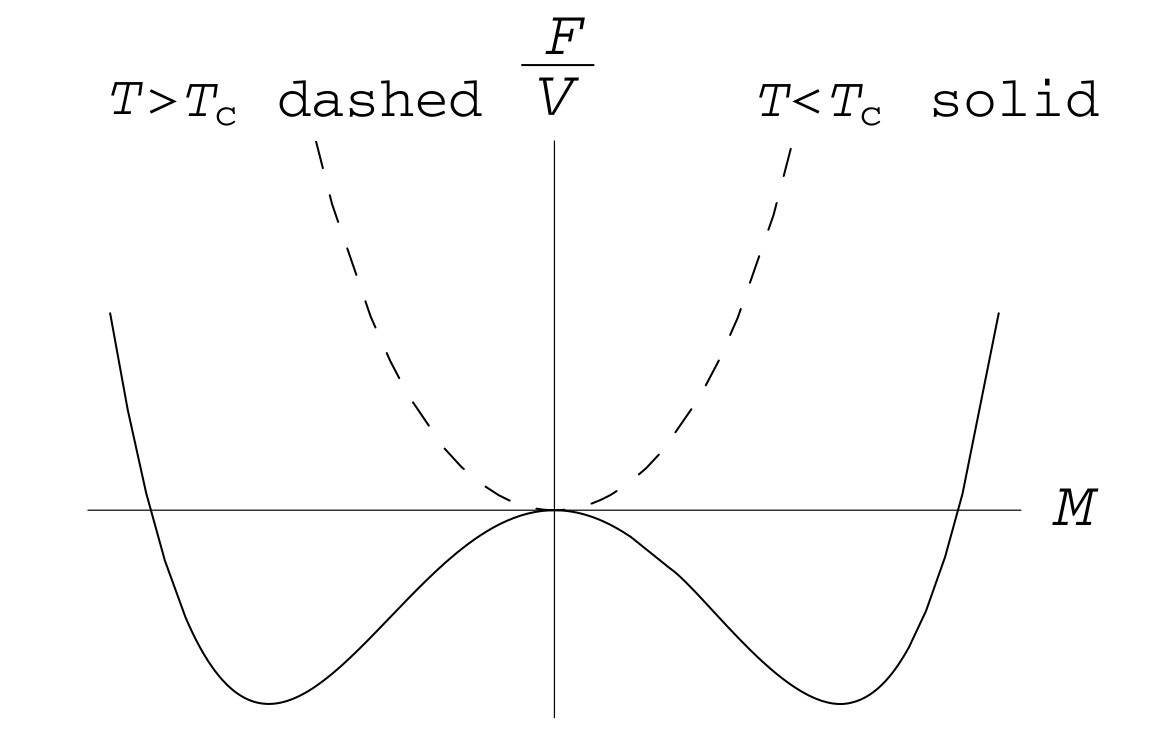
\includegraphics[scale=0.2]{SM/landau.png}
\caption{Landau free energy}
\end{figure}
\\
Furthermore, for $T = T_c$,
\[M_z^3 = \frac{B_z}{4b_0}\]
Finally we note that if $B_z$ is changed to $B_z + \delta B_z$, the corresponding equilibrium distribution $M_z$ can be written as $M_z + \delta M_z$. We thus get
\[2a_0(T-T_c)\delta M_z + 12b_0M_z^2\delta M_z = \delta B_z\]
Setting $B_z = 0$, we find
\[\chi = \left. \frac{\delta M_z}{\delta B_z} \right|_{B_z = 0} = \begin{cases} \frac{1}{2a_0(T-T_c)} \quad T>T_c \\ \frac{1}{4a_0(T_c-T)} \quad T<T_c \end{cases} \]
Landau's theory qualitatively reproduces the expected singular behaviour.
\\ \\
It is also possible to get a rather precise statement regarding long-range correlations within the framework of Landau's theory. Recall that
\[\delta M(\bm{y}) = \int d^3x C_T(|\bm{x}-\bm{y}|)\delta B(\bm{x})\]
From the equations which describe the equilibrium magnetization density we have with $c(T) = c_0$,
\[2a(T)M_z(\bm{x}) + 4b_0M_z^3(\bm{x})- 2c_0\nabla^2M_z(\bm{x}) = B_z(\bm{x})\]
So, we can get
\[[2a_0(T-T_c) + 12b_0M_z^2 - 2c_0\nabla^2] \delta M_z(\bm{x}) = \delta B_z(\bm{x})\]
From these equations it follows that
\[[2a_0(T-T_c) + 12b_0M_z^2 - 2c_0\nabla^2]C_T(|\bm{x} - \bm{y}|) = \delta(\bm{x} - \bm{y}) \]
Setting $B_z = 0$ and rescaling the coordinates as $(\bm{u},\bm{v}) = 2c_0(\bm{x},\bm{y})$ we get
\[[2\bar{a}_0(T-T_c) - \nabla^2] C_T(|\bm{u} - \bm{v}|) = \delta(\bm{u} - \bm{v})\]
where $\bar{a}_0 = a_0/(2c_0)^3$.
This result is valid in the region $T > T_c$ . For $T < T_c$ we get
\[[4\bar{a}_0(T_c-T) - \nabla^2] C_T(|\bm{u} - \bm{v}|) = \delta(\bm{u} - \bm{v})\]
The solution is
\[C_T(|\bm{x} - \bm{y}|) = \frac{1}{4\pi} \frac{e^{-\frac{|\bm{x} - \bm{y}|}{\xi}}}{|\bm{x} - \bm{y}|}\]
where $\xi^2 = c_0/a(T)$ for $T > T_c$ and $\xi^2 = -c_0/2a(T)$ for $T < T_c$.
We notice that $\xi \to \infty$ as $T \to T_c$. Thus Landau's theory is in qualitative agreement with the intuitive idea that long-range correlations are generated in a ferromagnet as $T \to T_c$.
\\
Another point to note is that if $\delta B_z$ were $\bm{x}$ independent, then as we saw before
\[\chi(0) = \frac{\delta M(0)}{\delta B} = \int d^3x C_T(|\bm{x}|) \sim \chi^2 \to \infty \quad \mbox{ as } T \to T_c\]
\\ \\
Let us summarize the results obtained from Landau's approach. The approach focused on long-range correlations and suggested that the singular behaviour of the susceptibility was due to such correlations when $T \to T_c$. 
The approach also predicts that the relation between different macroscopic parameters involves power laws,
\[M_z \sim (T_c - T)^{\beta} \quad T \to T_c\]
\[M_z \sim B_z^{1/\delta} \quad T = T_c\]
\[\chi \sim \frac{1}{(T_c-T)^{\gamma}} \quad T \to T_c\]
with $\beta = \frac{1}{2}$, $\gamma = 1$, and $\delta = 3$. The parameters $\beta$, $\delta$ and $\gamma$ are called critical exponents and are measured experimentally. 
The experimental values for these parameters
$\beta \approx 1.33$, $\delta \approx 4.5$, and $\gamma \approx 1.2$ are found for different ferromagnet with different lattice structures and widely differing values for the Curie temperature $T_c$. 
These parameters thus are a universal property of the ferromagnetic phase transition. This is also a feature of Landau's theory. Thus Landau's theory is in qualitative
agreement with experiment.

\section{Renormalization group}
\subsection{Introduction}
Although Landau's theory is in good qualitative agreement with experiment there is room for improvement on the quantitative level concerning the critical exponents.
Instead of considering a model for the free energy we now consider the partition function directly. 
\\
Let us consider a one-dimensional ferromagnetic system described in terms of an Ising model.
\[Z = \mathrm{Tr}e^{-\beta H}\]
with
\[H = -J\sum_{i=1}^N S_i S_{i+1} - H\sum_{i=1}^N S_i\]
where $S_i = \pm 1$ denotes the (uniaxial) magnetization or spin of site $i$ (periodic boundary conditions, $S_{N+1} = S_1$, imposed), and $H$ represents an external field. We have
\[e^{-\beta H} = e^{\sum_{1}^N KS_iS_{i+1} + hS_i} = \prod_{i=1}^N T(S_i,S_{i+1})\]
where $K = \beta J > 0$ and $h = \beta H$, and the weight is defined through the relation $T(S,S') = \exp[KSS' + \frac{h}{2}(S+S')]$. So,
\[Z = \sum_{\{S_i\}} e^{-\beta H} = \mathrm{Tr}T^N\]
and
\[T = \begin{pmatrix}
e^{K+h} & e^{-K} \\ e^{-K} & e^{K-h}
\end{pmatrix}\]
Following the program outlined by Kadanoff's seminal work on the foundations of the RG, we will follow a strategy whereby this renormalization step may be effected by subdividing the spin chain into regular clusters of b neighbouring spins. We may then proceed to sum over the $2b$ sub-configurations of each cluster, thereby generating an effective functional describing the inter-cluster energy balance. 
While it is clear that this energy functional exists, a far less obvious question to ask is whether it will again have the form of an effective Ising spin system. Remarkably, the answer is affirmative: the Ising model is said to be "renormalizable." 
The structural reproduction of the model implies that we can think of each cluster as some kind of meta-Ising spin, or block spin. More importantly, it guarantees that the renormalization step qualifies for iteration: in a second RG step, $b$ block spins are grouped to form a new cluster (now comprising $b^2$ of the microscopic spins) which are then traced out, etc. We have
\[Z_{N}(K,h) = \mathrm{Tr} T^N = \mathrm{Tr} (T^b)^{N/b} =\mathrm{Tr} (T')^{N/b} = Z_{N/b}(K',b')\]
Define $u \equiv e^{-K}$ and $v \equiv e^{-h}$, we can work out
\[u' = \frac{\sqrt{v+v^{-1}}}{(u^4 + u^{-4} + v^2 + v^{-2})^{1/4}} \quad v' = \frac{\sqrt{u^4 + v^2}}{\sqrt{u^4 + v^{-2}}}\]
The possibility of representing the new transfer matrix in the same algebraic structure as the old one implies that the transformed model again describes an Ising spin system. However, the Hamiltonian $\beta H$ of the new block spin system is defined at a different temperature, magnetic field and exchange constant and describes fluctuations on length scales that are twice as large as in the original system.
In particular, the short-distance cut-off has been doubled.
\\ \\
To make further progress, one may focus on the two relevant parameters $u'$ and $v'$ and observe that the result of the block spin transformation can be represented as a discrete map
\[\begin{pmatrix} u' \\ v' \end{pmatrix} = \begin{pmatrix}
f_1(u,v) \\ f_2(u,v)
\end{pmatrix} \]
In one-dimensional Ising model, the map $f$ possesses two
disjoint sets of fixed points $(u^*,v^*) = (0,1)$ and $(u^*,v^*) = (1,v)$.
\\
The set of fixed points represents the most important structural characteristic of an RG analysis. They organize the space of "flowing" coupling constants into sectors of qualitatively different behaviour. 
In particular, one may note that, at a fixed point, all characteristics of the model, including its correlation length $\xi$, remain invariant. 
On the other hand, we noticed above that an RG step is tantamount to doubling the fundamental length scale of the system. Consistency requires that either $\xi = 0$ or $\xi = \infty$. 
In the present case, the line of fixed points is identified with $u = \exp[-\beta J] = 1$, i.e. $\beta = 0$. 
This is the limit of infinitely large temperatures, at which we expect the model to be in a state of maximal thermal disorder, that is $\xi = 0$. 
Besides the high-temperature fixed line, there is a zero-temperature fixed point $(u, v) = (\exp[−\beta J], \exp[−\beta h]) = (0, 1)$ implying $T \to 0$ and $h \to 0$. Upon approaching zero temperature, the system is expected to order and to build up long-range correlations, $\xi \to \infty$. And we can say critical point corresponds to a fixed point of RG group with infinity correlation length.
\\
Notice, however, an important difference between the high- and the low-temperature set of fixed points: while the former is an attractive fixed point in the sense that the RG trajectories approach it asymptotically, the latter is a repulsive fixed point. No matter how low the temperature at which we start, the RG flow will drive us into a regime of effectively higher temperature or lower ordering. 
(Of course, the physical temperature does not change under renormalization. All we are saying is that the block spin model behaves as an Ising model at a higher temperature than the original system.)
\\
A detailed discussion of one-dimensional Ising model can be found in section 8.1 from \emph{Condensed Matter Field Theory (Alexander Altland \& Ben Simons)}. A discussion of a model with continuous configurations can be found in section 8.2 of the same book. The model implements RG by integrating out fields with high frequency modes. The same method can also be used in relativistic quantum  field theory. A detail discussion can be found in section 12.1 form \emph{An introduction to quantum field theory (M.E.Peskin \& D.V.Schroeder)}

\subsection{Gell-Mann-Low equations}
There are a number of methodologically different procedures whereby the set of flow equations can be obtained from the microscopic theory. Here, we formulate this step in a language adjusted to applications in statistical field theory as opposed to particle physics. While there is considerable freedom in the actual implementation of the RG procedure, all methods share the feature that they proceed in a sequence of three more or less canonical steps.
\subsubsection{Subdivision of the field manifold}
In the first step, one may decompose the integration manifold $\{\phi\}$ into a sector to be integrated out, $\{\phi_f\}$, and a complementary set, $\{\phi_s\}$.
\begin{itemize}
\item We may proceed according to a generalized block spin scheme and integrate over all degrees of freedom located within a certain structural unit in the base manifold $\{\bm{x}\}$.(This scheme is adjusted to lattice problems where $\{\bm{x}\} = \{\bm{x}_i\}$ is a discrete set of points.)
\item We could decide to integrate over a certain sector in momentum space. When this sector is defined to be a shell $\Lambda /b < |\bm{p}| < \Lambda$, one speaks of a momentum shell integration. Naturally, within this scheme, the theory will be explicitly cutoff-dependent at intermediate stages.
\item Alternatively, we may decide to integrate over all high-lying degrees of freedom $\lambda^{-1} \leq |\bm{p}|$.
In this case, we will of course encounter divergent integrals. An elegant way to handle these divergences is to apply dimensional regularization. Within this approach one formally generalizes from integer dimensions $d$ to fractional values $d \pm \epsilon$. 
One motivation for doing so is that the formal extension of the characteristic integrals appearing during the RG step to non-integer dimensions are finite. As long as one stays clear of the dangerous values $d = \mbox{ integer}$ one can then safely monitor the dependence of the integrals on the IR cutoff $\lambda^{-1}$.
\end{itemize}

\subsubsection{RG step}
The second part of the program is to actually integrate over short range fluctuations. This step usually involves approximations. 
In most cases, one will proceed by a so-called loop expansion, i.e. one organizes the integration over the fast field $\phi_f$ according to the number of independent momentum integrals -loops - that occur after the appropriate contractions.
\\
Following the procedure, an expansion over the fast degrees of freedom gives an action in which coupling constants of the remaining slow fields are altered. 
Notice that the integration over fast field fluctuations may  lead to the generation of "new" operators, i.e. operators that have not been present in the bare action. In such cases one has to investigate whether the newly generated operators are "relevant" in their scaling behaviour. 
If so, the appropriate way to proceed is to include these operators in the action from the very beginning (with an a priori undetermined coupling constant). One then verifies whether the augmented action represents a complete system, i.e. one that does not lead to the generation of operators beyond those that are already present. If necessary, one has to repeat this step until a closed system is obtained.

\subsubsection{Rescaling}
One next rescales frequency/momentum so that the rescaled field amplitude $\phi'$ fluctuates on the same scales as the original field $\phi$, i.e. one sets
\[q \to bq \quad \omega \to b^z \omega\]
Here, the frequency renormalization exponent or dynamical exponent $z$ depend on the effective dispersion relating
frequency and momentum. 
We finally note that the field $\phi$, as an integration variable, may be rescaled arbitrarily. Using this freedom, we select a term in the action which we believe governs the behaviour of the "free" theory - in a theory with elastic coupling this might be the leading-order gradient operator $\int d^d r (\nabla \phi)^2$ - and require that it be strictly invariant under the RG step. 
To this end we designate a dimension $L^{d_{\phi}}$ for the field, chosen so as to compensate for the factor $b^x$ arising after the renormalization of the operator. The rescaling $\phi \to b^{d_{\phi}}$ is known as field renormalization. It renders the "leading" operator in the action scale invariant.
\\ \\
As a result of all these manipulations, we obtain a renormalized action
\[S[\phi] = \sum_a g'_a \mathcal{O}_a[\phi]\]
which is entirely described by the set of changed coupling constants, i.e. the effect of the RG step is fully encapsulated in the mapping
\[\bm{g}' = \tilde{R}(\bm{g})\]
relating the old value of the vector of coupling constants to the renormalized one. 
By letting the control parameter, $l \equiv \ln b$, of the RG step assume infinitesimal values, one can make the difference between bare and renormalized coupling constants
arbitrarily small. 
It is then natural to express the difference in the form of a generalized $\beta$-function or Gell-Mann-Low equation
\[\frac{d\bm{g}}{dl} = R(\bm{g})\]
where the right-hand side is defined through the relation
\[R(\bm{g}) = \lim_{l \to 0} l^{-1} (\tilde{R}(\bm{g}) - \bm{g})\]
\\
Actually Gell-Mann-Low equation here is the same equation as the one in relativistic quantum field theory which describe the flow of coupling coefficient with the energy scale of the experiment. Suppose the cutoff of the theory is $\Lambda_0$, the energy scale of the experiment is $\mu$, and $\lambda_i$ is the coupling coefficient in the theory with dimension $[\mbox{energy}] ^{d_{i}}$. If the dimension of the physical quantity we want to measure is $d_Q$, then generally, we have
\[\frac{Q}{\Lambda_0^{d_O}} = F(\frac{\mu}{\Lambda_0},\frac{\lambda_i}{\Lambda_0^{d_i}})\]
Then, we can integrate out the high frequency mode between $\mu$ and $\Gamma_0$ of the theory and rescale the energy and momentum to get the new coupling coefficient $\lambda(b)$, where $b = \Lambda_0 / \mu$. So, in the new effective theory, we have
\[\frac{Q}{\mu^{d_O}} = F(1,\frac{\lambda_i(\Lambda_0 / \mu)}{\mu^{d_i}})\]
The flow of coupling coefficient given by
\[\frac{d\lambda}{d\ln \mu} = - \frac{d\lambda}{d\ln b}\]

\subsection{Analysis of the Gell-Mann-Low equation}
The prime structural characteristic of the Gell-Mann-Low equations is the set of fixed points, i.e. the submanifold $\{\bm{g}^*\}$ of points in coupling constant space which are stationary under the flow. 
Once the coupling constants are fine-tuned to a fixed point, the system no longer changes under subsequent RG transformations. In particular it remains invariant under the change of space/time scale associated with the transformation.
Alluding to the fact that they look the same no matter how large a magnifying glass is used, systems with this property are referred to as self-similar.
\\
Now, to each system, one can attribute at least one intrinsic length scale, namely the length $\xi$ determining the exponential decay of field correlations. 
However, the existence of a finite, and pre-determined, intrinsic length scale clearly does not go together with invariance under scale transformations. We thus conclude that, at a fixed point, either $\xi = 0$ (not so interesting), or $\xi = \infty$. 
However, a diverging correlation length $\xi \to \infty$ is a hallmark of a second-order phase transition. We thus tentatively identify fixed points of the RG flow as candidates for "transition points" of the physical system.
\\
This being so, it is natural to pay special attention to
the behaviour of the flow in the immediate vicinity of the fixed-point manifolds. If the set of coupling constants, $g$, is only close enough to a fixed point, $g^*$, it will be sufficient to consider the linearized mapping
\[R(\bm{g}) \equiv R[g^*+(g-g^*)] \approx W(g-g^*) \quad W_{ab} = \left. \frac{\partial R_a}{\partial g_b} \right|_{g=g^*}\]
To explore the properties of flow, let us assume that we had managed to diagonalize the matrix $W$ . Denoting the eigenvalues by $\lambda_{\alpha}$, and the left-eigenvectors by $\phi_{\alpha}$, we have
\[\phi_{\alpha}^T W = \phi_{\alpha}^T\lambda_{\alpha}\]
let $v_{\alpha}$ be the $\alpha$th component of the vector $\bm{g} - \bm{g}^*$ when represented in the basis $\{\phi_{\alpha}\}$:
\[v_{\alpha} = \phi_{\alpha}^T (\bm{g}-\bm{g}_{*})\]
We can easily derive that
\[\frac{dv_{\alpha}}{dl} = \lambda_{\alpha}v_{\alpha}\]
Under renormalization, the coefficients $v_{\alpha}$ change by a mere scaling factor $\lambda_{\alpha}$, wherefore they are called scaling fields.
\[v_{\alpha}(l) \sim \exp(l\lambda_{\alpha})\]
This result suggests a discrimination between at least three different types of scaling fields
\begin{itemize}
\item For $\lambda_{\alpha} > 0$ the flow is directed away from the critical point. The associated scaling field
is said to be relevant (in the sense that it forcefully drives the system away from the critical region).
\item In the complementary case, $\lambda_{\alpha} < 0$, the flow is attracted by the fixed point. Scaling fields
with this property are said to be irrelevant.
\item Finally, scaling fields which are invariant under the flow, $\lambda_{\alpha} = 0$ , are termed marginal.
\end{itemize}
The distinction of relevant/irrelevant/marginal scaling fields in turn implies a classification of different types of fixed points:
\begin{itemize}
\item Firstly, there are stable fixed points, i.e. fixed points whose scaling fields are all irrelevant or, at worst, marginal. 
These points define what we might call "stable phases of
matter": when you release a system somewhere in the parameter space surrounding any of these attractors, it will scale towards the fixed point and eventually sit there. Or,
expressed in more physical terms, looking at the problem at larger and larger scales will make it more and more resemble the infinitely correlated self-similar fixed-point configuration. (Recall the example of the high-temperature fixed line of the one-dimensional Ising
model encountered earlier.) 
By construction, the fixed point is impervious to moderate
variations in the microscopic morphology of the system, i.e. it genuinely represents what one might call a "state of matter."
\item Complementary to stable fixed points, there are unstable fixed points. Here, all scaling fields are relevant (the $T = 0$ fixed point of the 1-D Ising model). These fixed points represent the concept of a Platonic ideal: you can never get there and, even if you managed to approach it closely, the harsh conditions of reality will make you flow away from it.
Although unstable fixed points do not correspond to realizable forms of matter, they are of importance inasmuch as they "orient" the global RG flow of the system.
\item Finally, there is the generic class of fixed points with both relevant and irrelevant scaling fields. These points are of particular interest inasmuch as they can be associated with phase transitions. 
To understand this point, we first note that the $r$ eigenvectors $\phi_{\alpha}$ associated with irrelevant scaling fields span the tangent space of an $r$-dimensional
manifold known as the critical surface. 
This critical manifold forms the basin of attraction of the fixed point, i.e. whenever a set of physical coupling constants $g$ is fine-tuned so that $g \in S$, the
expansion in terms of scaling fields contains only irrelevant contributions and the system will feel attracted to the fixed point as if it were a stable one.
\\
However, the smallest deviation from the critical surface introduces a relevant component driving the system exponentially away from the fixed point.For example, in the
case of the ferromagnetic phase transition  deviations from the critical temperature $T_c$ are relevant. 
\\
If we consider a system only slightly above or below $T_c$, it may initially appear to be critical. However, upon further increasing the scale, the relevant deviation will grow and drive the system away from criticality, either towards the stable high-temperature fixed point of the paramagnetic phase or towards the ferromagnetic low-temperature phase.
\end{itemize}

\section{Critical exponents}
The most fundamental signature of a phase transition is its order parameter, a quantity whose value unambiguously identifies the phase of the system. Transitions between different phases of matter fall into two large categories. 
In first-order phase transitions the order parameter exhibits a discontinuous jump across the transition line.
In the complementary class of second-order transitions, the order parameter changes in a non-analytic but continuous manner.
\\ 
The phenomenology of second-order transitions is generally richer than that of first-order transitions. 
As a thermodynamic state variable, the order parameter $M$ is coupled to a conjugate field, $H = -\partial_H F$, where $F$ is the free energy. 
At a second-order transition, $M$ changes non-analytically, which means that the second-order derivative, a thermodynamic susceptibility,$\chi = -\partial_H^2 F$ , develops a singularity. 
Now, you may recall that the susceptibility is intimately linked to the field fluctuation behaviour of the system. A divergence of the susceptibility implies the accumulation of infinitely long-range field fluctuations.
\\
The divergence of the susceptibility goes hand in hand with non-analytic and/or singular behaviour of all sorts of other physical quantities. In fact, an even stronger statement can be made.
We have seen that, right at the transition/fixed point, the system is self-similar. This implies that the behaviour of its various characteristics must be described by power laws.
The set of different exponents characterizing the relevant power laws occurring in the vicinity of the transition are known as critical exponents.
\\
In the following, let us briefly enumerate the list of the most relevant exponents, $\alpha$, $\beta$, $\gamma$, $\delta$, $\eta$ and $\nu$. 
Although we shall again make use of the language of the magnetic transition, it is clear that the definitions of most exponents generalize to other systems.
\begin{enumerate}
\item In the vicinity of the critical temperature, the specific heat $C = -T\partial_T^2 F$ scales as $C \sim |t|^{-\alpha}$, where $t = (T-T_c)/T_c$ measures the distance to the critical point. 
\\
Note that, by virtue of this definition, a non-trivial statement has been made: although the phases above and below the transition are essentially different, the scaling exponents controlling the behaviour of C are identical. The same applies to most other exponents listed below.
\item Approaching
the transition temperature from below, the magnetization vanishes as
\[M \equiv -\left. \partial_H F \right|_{H \searrow 0} \sim (-t)^{\beta} \]
\item The magnetic susceptibility behaves as
\[\chi \equiv -\left. \partial_h M \right|_{h \searrow 0} \sim (-t)^{-\gamma} \]
\item At the critical temperature, $t = 0$, the field dependence of the magnetization is given by $M \sim |h|^{1/\delta}$
\item Upon approaching the transition point, the correlation length diverges as $\xi \sim |t|^{-\nu}$
\item The correlation function,
\[C(\bm{r}) \sim \begin{cases} \frac{1}{|\bm{r}|^{d-2+\eta}} \quad |\bm{r}| \ll \xi \\ \exp[-|\bm{r}|/\xi] \quad |\bm{r}| \gg \xi  \end{cases} \]
crosses over from exponential to a power law scaling behaviour at the length scale $\xi$. 
To motivate the power, one may notice that $C \sim \langle \phi \phi \rangle$ carries twice the dimension of the field $\phi$. 
The engineering dimension of the latter follows from the requirement that the gradient operator $\sim \int d^dr (\nabla \phi)^2$ be dimensionless: $[\phi] = L^{(2-d)/2}$, according to which $C(r)$ has canonical dimension $L^{2-d}$ . 
The exponent $\eta$, commonly referred to as the anomalous dimension of the correlation function, measures the mismatch between the observed and the canonical dimension.
\end{enumerate}

\subsubsection{Universality}
In fact, the majority of critical systems can be classified into a relatively small number of universality classes. Crudely speaking, leaving apart more esoteric classes of phase transitions there are $\mathcal{O}(10)$ fundamentally different types of flow recurrently appearing in practical applications. This has to be compared with the near infinity of different physical systems that display critical phenomena. The origin of this universality can readily be understood from the concept of critical surfaces.
\\ \\
Imagine, then, an experimentalist exploring a system that is known to exhibit a phase transition. Motivated by the critical phenomena that accompany phase transitions, the available control parameters $X_i$ (temperature, pressure, magnetic field, etc.) will be varied until the system begins to exhibit large fluctuations. On a theoretical level, the variation of the control parameters determines the initial values of the coupling constants of the model (as they functionally depend on the $X_i$s through their connection to the microscopic Hamiltonian). For microscopic parameters corresponding to a point above or below the critical manifold, the system asymptotically (i.e. when looked at at sufficiently large scales) falls into either the "high-" or the "low-temperature" regime. 
However, eventually the trajectory through parameter space will intersect the critical surface. For this particular set of coupling constants, the system is critical. As we look at it on larger and larger length scales, it will be attracted by the fixed point at S, i.e. it will display the universal behaviour characteristic of this particular point. 
This is the origin of universality: variation of the system parameters in a different manner (or for that matter considering a second system with different material constants) will generate a different trajectory. 
However, as long as this trajectory intersects with S, it is guaranteed that the critical behaviour will exhibit the same universal characteristics (controlled by the unique fixed point).
\\ \\
In fact a more far-reaching statement can be made. Given that there is an infinity of systems exhibiting transition behaviour while there is only a very limited set of universality classes, many systems of very different microscopic morphology must have the same universal behaviour. More formally, different microscopic systems must map onto the same critical low-energy theory.

\subsubsection{Scaling}
Let us consider the case of the ferromagnetic transition, i.e. a transition we have characterized in terms of six critical exponents. 
However, the flow in the vicinity of the magnetic fixed point is controlled by only two relevant scaling fields, the (reduced) temperature $t \equiv (T-T_c)/T$ and the reduced magnetic field $h \equiv H/T$. Other scaling fields $g_i$s are irrelevant.
Under a renormalization group transformation, the reduced free energy $f = F/TL^d$ will behave as
\begin{eqnarray}
f(t,h,g_i) &=& b^{-d}f(tb^{y_t}, hb^{y_h},g_ib^{\lambda_i}) = t^{d/y_t} f(1,ht^{-y_h/y_t},g_it^{-\lambda_i/y_t}) \nonumber \\ 
&\overset{t\ll1}{\approx}& t^{d/y_t} f(1,ht^{-y_h/y_t},0) \equiv t^{d/y_t}\tilde{f}(ht^{-y_h/y_t}) \nonumber
\end{eqnarray}
Here, we have used the freedom of arbitrarily choosing the parameter $b$ to set $tb^{y_t} = 1$ while, in the third equality, we have assumed that we are sufficiently close to the transition that the dependence of $f$ on irrelevant scaling fields is inessential.
Comparing with the definitions of critical exponent, it is straightforward to show that
\[\alpha = 2 - \frac{d}{y_t} \quad \beta = \frac{d-y_h}{y_t} \quad \gamma = \frac{2y_h-d}{y_t} \]
\[\delta = \frac{y_h}{d - y_h} \quad \nu = \frac{1}{y_t} \quad \eta = 2 + d - 2y_h\]
The dimensions of the relevant scaling fields have a more fundamental status than the critical exponents.
Of the six classical exponents, only two can be truly
independent. It is straight forward to derive the scaling laws by eliminating $y_h$ and $y_t$:
\[\nu(2-\eta) = \gamma \quad \alpha + 2\beta + \gamma = 2 \quad \beta(\delta - 1) = \gamma \quad 2 - \alpha = \nu d\]

\section{RG analysis of the ferromagnetic transition}
\subsection{Preliminary dimensional analysis}
We now turn to the problem of calculating the various critical exponents of ferromagnetic system. The method presented here will improve on Landau's theory while reducing to the latter in a certain limit. The idea is to represent Landau's model as a certain approximation to the partition function of some quantum field theory for the order parameter. 
We suppose the partition function of Ising model can be represented by
\[Z = \int \mathcal{D}\phi e^{-S[\phi]}\]
with 
\[S[\phi] = \int d^d x \left[\frac{1}{2}(\nabla \phi)^2 + \frac{r}{2}\phi^2 + \frac{\lambda}{4!}\phi^4 - h\phi \right]\]
The functional integral above is not derived from a concrete Hamiltonian. The path integral should be understood rather as a statistical averaging over different configurations of the order parameter $\phi(x)$. 
\\
The reason why it it possible to neglect both higher powers and gradients of the field $\phi$ that are surely present in the exact reformulation of the Ising problem in terms of $\phi$-variables can be formulated by dimensional analysis.
Anticipating that the "real" dimensions carried by the operators in the action will be not too far from their
engineering dimensions, we begin by exploring the latter. 
It is straightforward to attribute engineering dimensions to all operators:
\[\left[\phi^2 \right] = L^2 \quad \left[\phi^4 \right] = L^{4-d} \quad \left[\phi^{2n} \right] = L^{d + (2-d)n/2} \quad  \left[(\nabla^m \phi)^2 \right] = L^{2(1-m)}\]
These relations convey much about the potential significance of all structurally allowed operators:
\begin{itemize}
\item The engineering dimension of the non-gradient operator $\sim \phi^2$ is positive in all dimensions, indicating general relevance.
\item The $\phi^4$ operator is relevant (irrelevant) in dimensions $d < 4 (d > 4)$. This suggests that for $d > 4$ a harmonic approximation $(\lambda = 0)$ of the model should be reasonable. 
It also gives us a preliminary clue as to how we might want to approach the $\phi^4$-model on a technical level: 
while for dimensions "much" smaller than $d = 4$ the interaction operator $\sim \phi^4$ is strongly relevant, the dimension $d = 4$ itself is borderline. 
This suggests that we analyze the model at $d = 4$, or maybe "close"  to $d = 4$ where the $\phi^4$ operator is not yet that virulent, and then try to extrapolate to infer what happens at the "physical dimensions" of $d = 2$ and $3$.
\item Operators $\phi^{n > 4}$ become relevant only in dimensions $d < \frac{2}{1-2/n} < 4$. 
However, even below these threshold dimensions, operators of high powers in the field variable are much less relevant than the dominant non-harmonic operator $\phi^4$. This is the a posteriori justification for the neglect of $\phi^{n>4}$ operators in the derivation of the model.
\item Similarly, operators with more than two gradients are generally irrelevant and can be neglected in all dimensions
\item In contrast, the operator $\phi$ coupling to the magnetic field carries dimension $(1+d/2)$ and is therefore always strongly relevant.
\end{itemize}

\subsection{Landau mean-field theory}
We can approximate $S[\phi]$ by its functional Taylor expansion about $\phi_0$, which, in turn, is defined by the condition $\delta S \delta \phi = 0$. Thus
\[S[\phi] = S[\phi_0] + \frac{1}{2!} \int d^dx \int d^dy (\phi-\phi_0)_x (\phi-\phi_0)_y \left( \frac{\delta^2 S}{\delta \phi_x \delta \phi_y} \right)_{\phi_0}\]
First let us consider the classical approximation to the partition function $Z$. Approximating the functional integral by its saddle point we find
\[Z \approx e^{-S[\phi_0]}\]
On the other hand we have in the canonical ensemble
\[Z = e^{-\beta F}\]
Thus we can identify the free energy of statistical mechanics with $S[\phi_0]$ of our field theory
\[F = \frac{1}{\beta} S(\phi_0)\]
Landau mean-field theory can be seen as the "classical limit" or saddle point approximation of full path integral.

\subsection{Gaussian model}
As a first improvement on the mean-field approximation, let us explore the effect of quadratic fluctuations around the constant field configuration $\bar{\phi}$ Approaching the transition point from above, we set $\bar{\phi} = 0$ and approximate the action through its quadratic expansion
\[S[\phi] \approx \int d^dr \left[ \frac{r}{2}\phi^2 + \frac{1}{2}(\nabla\phi)^2- h\phi \right]\]
We split our field into fast and slow degrees of freedom $\phi = \phi_s + \phi_f$ resulting in the fragmentation of the action $S[\phi_s,\phi_f] = S_s(\phi_s) + S_f[\phi_f] + S_c[\phi_s,\phi_f]$. 
However, the crucial simplification, characteristic of a Gaussian theory, is that the action $S_c$ coupling fast and slow components vanishes, implying that the integration over the fast field merely leads to an inessential constant. 
\\
The effect of the RG step on the action is then entirely contained in the rescaling of the slow action. The scaling factors are determined by the engineering dimensions of the operators appearing in the action, i.e. $r \to b^2r$ and $h \to b^{1+d/2}h$. Using the fact that $r \sim t$ we can then readily write down the two relevant scaling dimensions of the problem, $y_t = 2$ and $y_h = d/2 + 1$. Finally, we have
\[\alpha = 2 - \frac{d}{2} \quad \beta = \frac{d}{4} - \frac{1}{2} \quad \gamma = 1 \quad \delta = \frac{d+2}{d-2} \quad \nu = \frac{1}{2} \quad \eta = 0\]
We note that the Gaussian model possesses only one fixed
point, namely $r = h = 0$, which in the context of $\phi^4$-theory is called the Gaussian fixed point.

\subsection{Renormalization group analysis}
Recall the  $\phi^4$ quantum field theory in $(d-1) + 1$-dimensional space-time. We have
\[Z = e^{iS_L[\phi]}\]
with
\[S_L = \int dt \int dx^3 \left[(\partial_t \phi)^2 - (\nabla \phi)^2 - \frac{r}{2}\phi^2 -h \phi \right]\]
If we replace $t$ by $-i\tau$, $Z$ will be exactly partition function of Ising model in $d$-dimensional space. For example, We can get the free propagator of statistical field theory by comparison with quantum field theory
\[D(p) = \frac{1}{p^2+r}\]
Note in calculation of loop integrals in quantum field theory, the free propagator will be the same as that in statistical field theory after Wick rotation. We may infer the renormalization group equation will be the same in these two cases. 
\\
The detailed calculation of flow equation in statistical field theory by the method of integrating out fast field can be found in section 8.4.4 of \emph{Condensed Matter Field Theory (Alexander Altland \& Ben Simons)}. The calculation in quantum field theory can be found in section 12.5 of \emph{An introduction to quantum field theory (M.E.Peskin \& D.V.Schroeder)}. Here, we list the final result.
\begin{eqnarray}
\frac{dr}{d\ln l} &=& 2r + \frac{\lambda}{16 \pi^2} - \frac{r\lambda}{16\pi^2} \nonumber \\
\frac{d\lambda}{d\ln l} &=& \epsilon \lambda - \frac{3\lambda^2}{16\pi^2} \nonumber \\
\frac{dh}{d\ln l} &=& \frac{6 - \epsilon}{2} \nonumber
\end{eqnarray}
where $\epsilon = 4-d$.
These equations clearly illustrate the meaning of the $\epsilon$-expansion. According to the second equation, a perturbation away from the Gaussian fixed point will initially grow at a rate set by the engineering dimension $\epsilon$. While, on the level of the classical, zero-loop theory, $\lambda$ would grow indefinitely, the one-loop contribution $\sim \lambda^2$ stops the flow at a value $\lambda \sim \epsilon$.
\\
Equating the right-hand sides of Gell-Mann-Low equations to zero (and temporarily ignoring the magnetic field), we indeed find that besides the Gaussian fixed point a non-trivial fixed point $(r_2^*, \lambda_2^*) = (-\frac{1}{6}\epsilon, \frac{16\pi^2}{3}\epsilon)$ has appeared.
Notice that the second fixed point is $\mathcal{O}(\epsilon)$ and coalesces with the Gaussian fixed point as $\epsilon$ is sent to zero. Plotting the $\beta$-function for the coupling constant $\lambda$, we further find that, for $\epsilon > 0$, $\lambda$ is relevant around the Gaussian fixed point but irrelevant at the non-trivial fixed point.
\begin{figure}[!h]
\centering
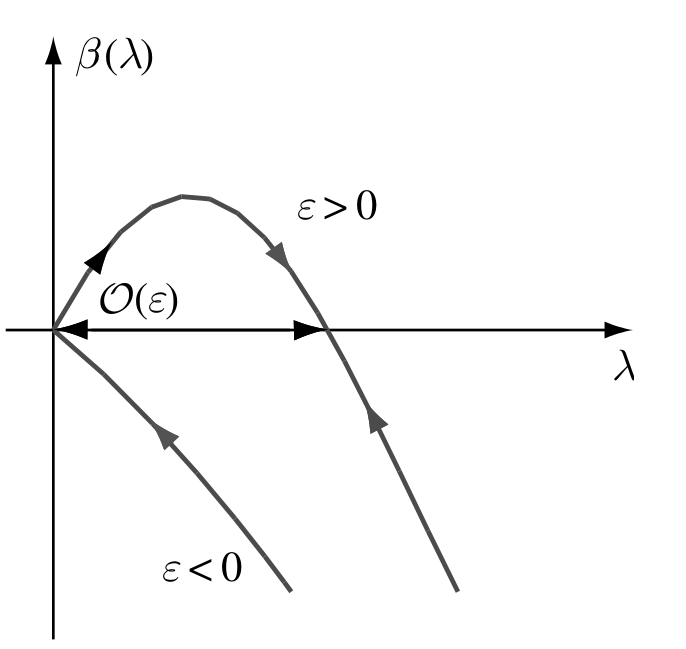
\includegraphics[scale=0.2]{/SM/RG1.png}
\caption{Beta function for $\lambda$}
\end{figure}
\\
To understand the full flow diagram of the system, one may linearize the $\beta$-function around both the Gaussian and the non-trivial fixed point. Denoting the linearized mappings by $W_{1,2}$ , we find
\[W_1 = \begin{pmatrix} 2 & \frac{1}{16\pi^2} \\ 0 & \epsilon \end{pmatrix} \quad W_2 = \begin{pmatrix} 2 - \frac{1}{3}\epsilon & \frac{1+ \frac{\epsilon}{6}}{16\pi^2}\\  0 & -\epsilon \end{pmatrix} \]
\\
Figure below shows the flow in the vicinity of the two fixed points, as described by the matrices $W_{1,2}$ as well as the extrapolation to a global flow chart.
\\
Notice that the critical surface of the system - the straight line interpolating between the two fixed points - is tilted with respect to the $r \sim$ temperature axis of the phase diagram. 
This implies that it is not the physical temperature alone that decides whether the system will eventually wind up in the paramagnetic or ferromagnetic sector of the phase diagram. 
Rather one has to relate temperature to the strength of the non-linearity to decide on which side of the critical surface we are. 
For example, for strong enough $\lambda$, even a system with $r$ initially negative may eventually flow towards the disordered phase. This type of behaviour cannot be predicted from the mean-field analysis of the model. Rather it represents a non-trivial effect of fluctuations.
\\
Finally notice that, while we can formally extend the flow into the lower portion of the diagram, $\lambda < 0$, this region is actually unphysical. The reason is that, for $\lambda < 0$, the action is fundamentally unstable and, in the absence of a sixth-order contribution, does not describe
a physical system.
\begin{figure}[!h]
\centering
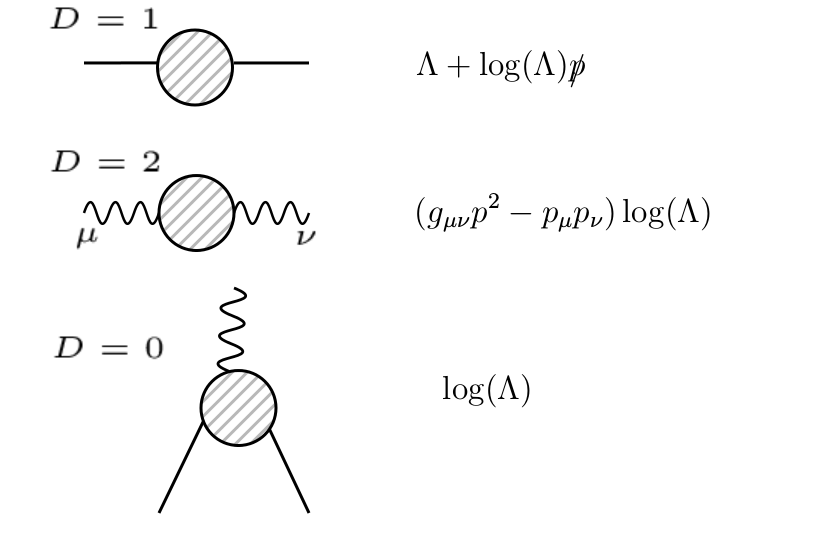
\includegraphics[scale=0.2]{/SM/RG2.png}
\caption{Phase diagram of the $\phi^4$-model as obtained from the $\epsilon$-expansion.}
\end{figure}
\\
Of the two eigenvalues of $W_2$, $2 - \frac{1}{3}\epsilon$ and $-\epsilon$, only the former is relevant. As with the Gaussian fixed point, it is tied to the scaling of the coupling constant $r \sim t$ and we have $y_t = 2 - \frac{1}{\epsilon}$ and, as before, $y_h = \frac{6-\epsilon}{2}$. Finally, we have critical exponents
\[\alpha = \frac{\epsilon}{6} \quad \beta = \frac{1}{2} - \frac{\epsilon}{6} \quad \gamma = 1 + \frac{\epsilon}{6} \quad \delta = 3 + \epsilon \quad \nu = \frac{1}{2} + \frac{\epsilon}{12} \quad \eta = 0\]
If we extend the radius of the expansion to $\epsilon = 1$,
we obtain the critical exponents for 3-dimensional Ising model. The agreement with the experimental results has improved even in spite of the fact that we have driven the $\epsilon$-expansion well beyond its range of applicability.











\end{document}